\subsection{Ridge regression}

Now we applied the ridge regression to perform variable selection. In \Fig~\ref{fig:RidgeCoefVsLambda} is shown the coefficients' behavior as $\lambda$ increases. 

\begin{figure}[h]
	\centering
	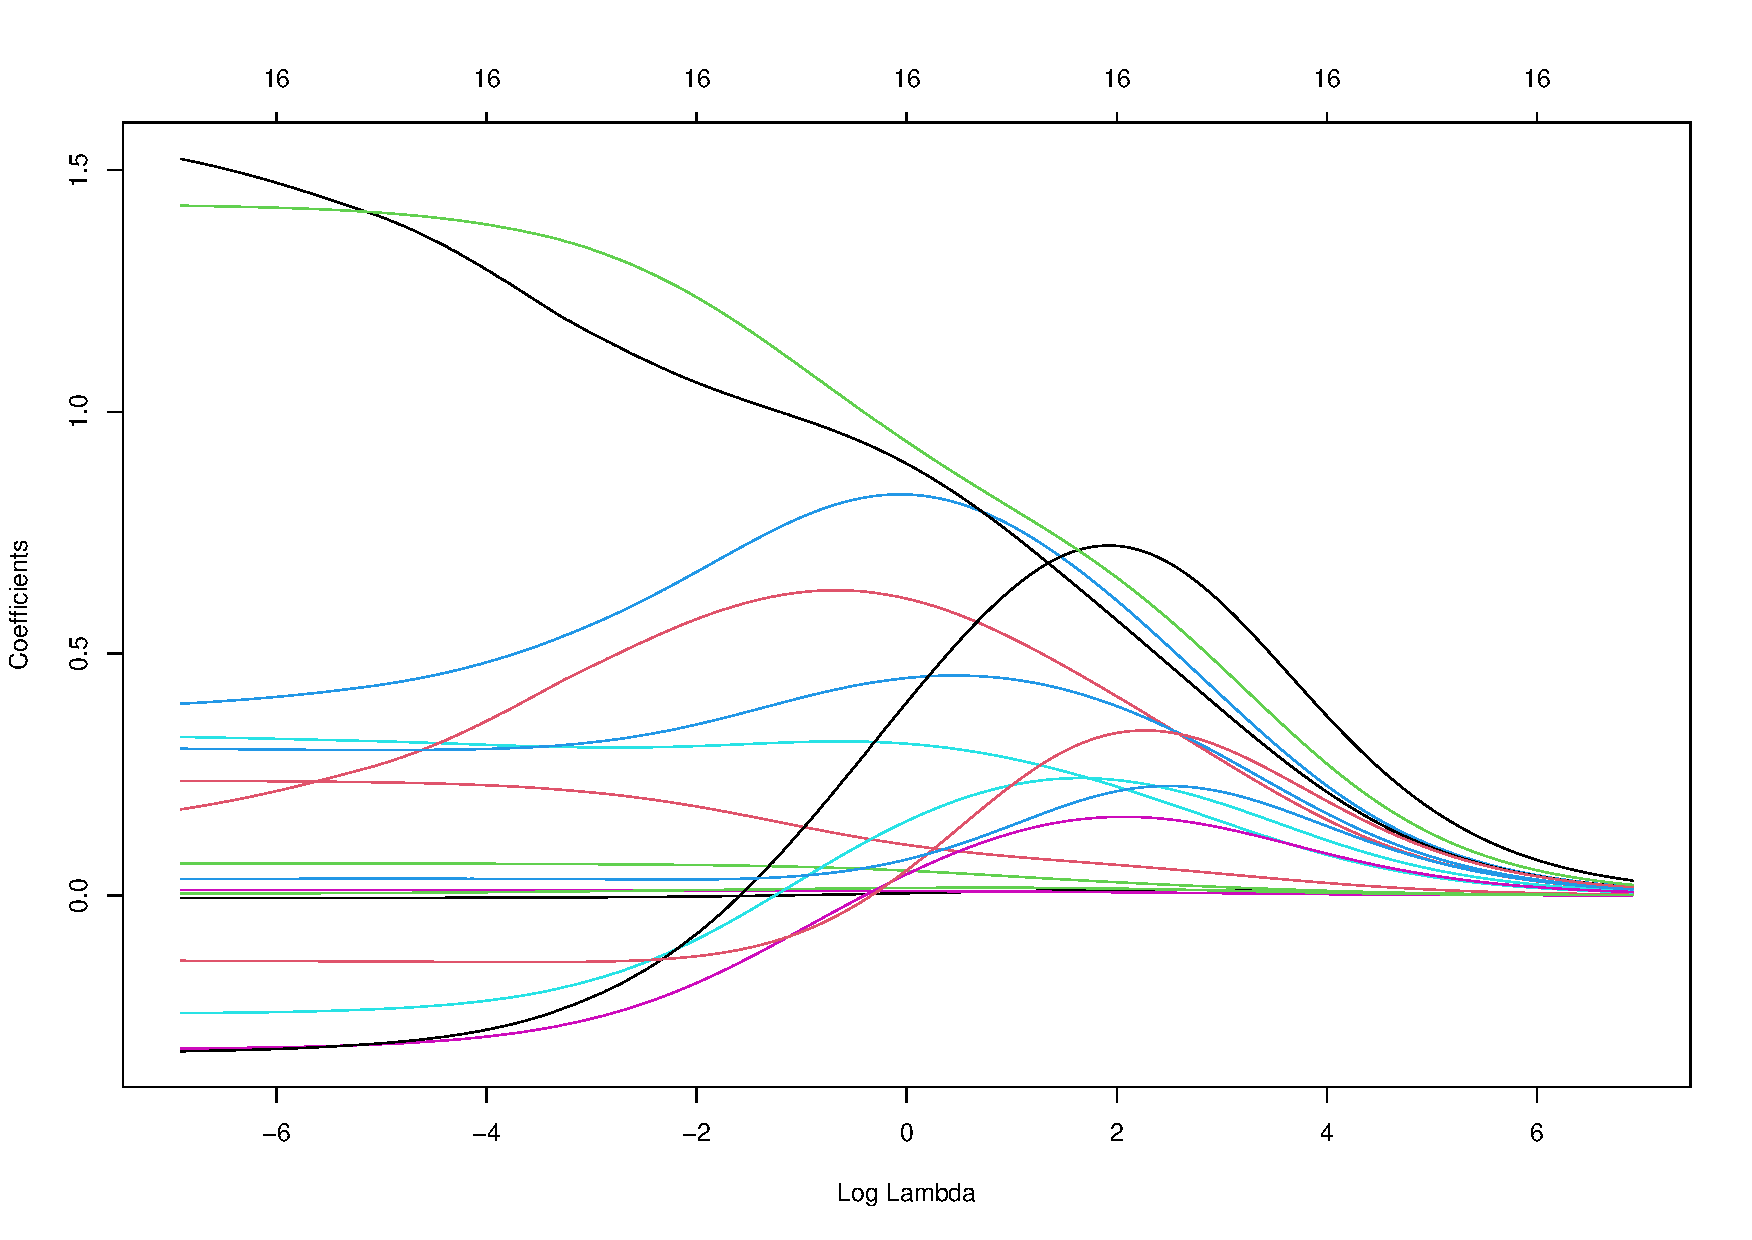
\includegraphics[width=0.4\linewidth]{ImageFiles/Regression/Ridge/RidgeCoefVsLambda.pdf}
	\caption{Ridge regression coefficients as function of $\lambda$.}
	\label{fig:RidgeCoefVsLambda}
\end{figure}

It is possible to observe that for enough large values of $\lambda$, around $10^2$, all the coefficients tend to become close to zero. However, they are never exactly zero.

To select the optimal value of the penalization factor $\lambda$ we employed \textit{k}-fold cross-validation with $\textit{k}=10$. In \Fig~\ref{fig:RidgeCvPlot} it is possible to observe the trend of the cross-validated mean square error (MSE) when $\lambda$ increases. The optimal value was found to be $\lambda_{opt} = 0.0268$.

\begin{table}[H]
	\centering
	\begin{tabular}{|| l | r ||} 
		\hline
		\multicolumn{2}{|c|}{Equation} \\
		\hline
		Variable & Coefficient \\
		\hline
		intercept & -3.9290 \\
		GP & -0.0045 \\
		MIN & 0.2320 \\
		FG\% & 0.0641 \\
		3P MADE & 0.7084 \\
		3PA & 0.2088 \\
		3P\% & 0.0104 \\
		FTM & 1.3534 \\
		FTA & 0.3384 \\
		FT & 0.0052 \\
		OREB & 0.2031 \\
		DREB & -0.2163 \\
		AST & -0.3492 \\			
		STL & -0.2449 \\
		BLK & -0.1653 \\
		TOV & 1.4755 \\
		TARGET\_5Yrs & 0.0657 \\				
		\hline
	\end{tabular}
	\caption{Ridge regression coefficients with $\lambda_{opt}$.}
	\label{table:FinalRidgeCoef}
\end{table}


\begin{figure}[H]
	\centering
	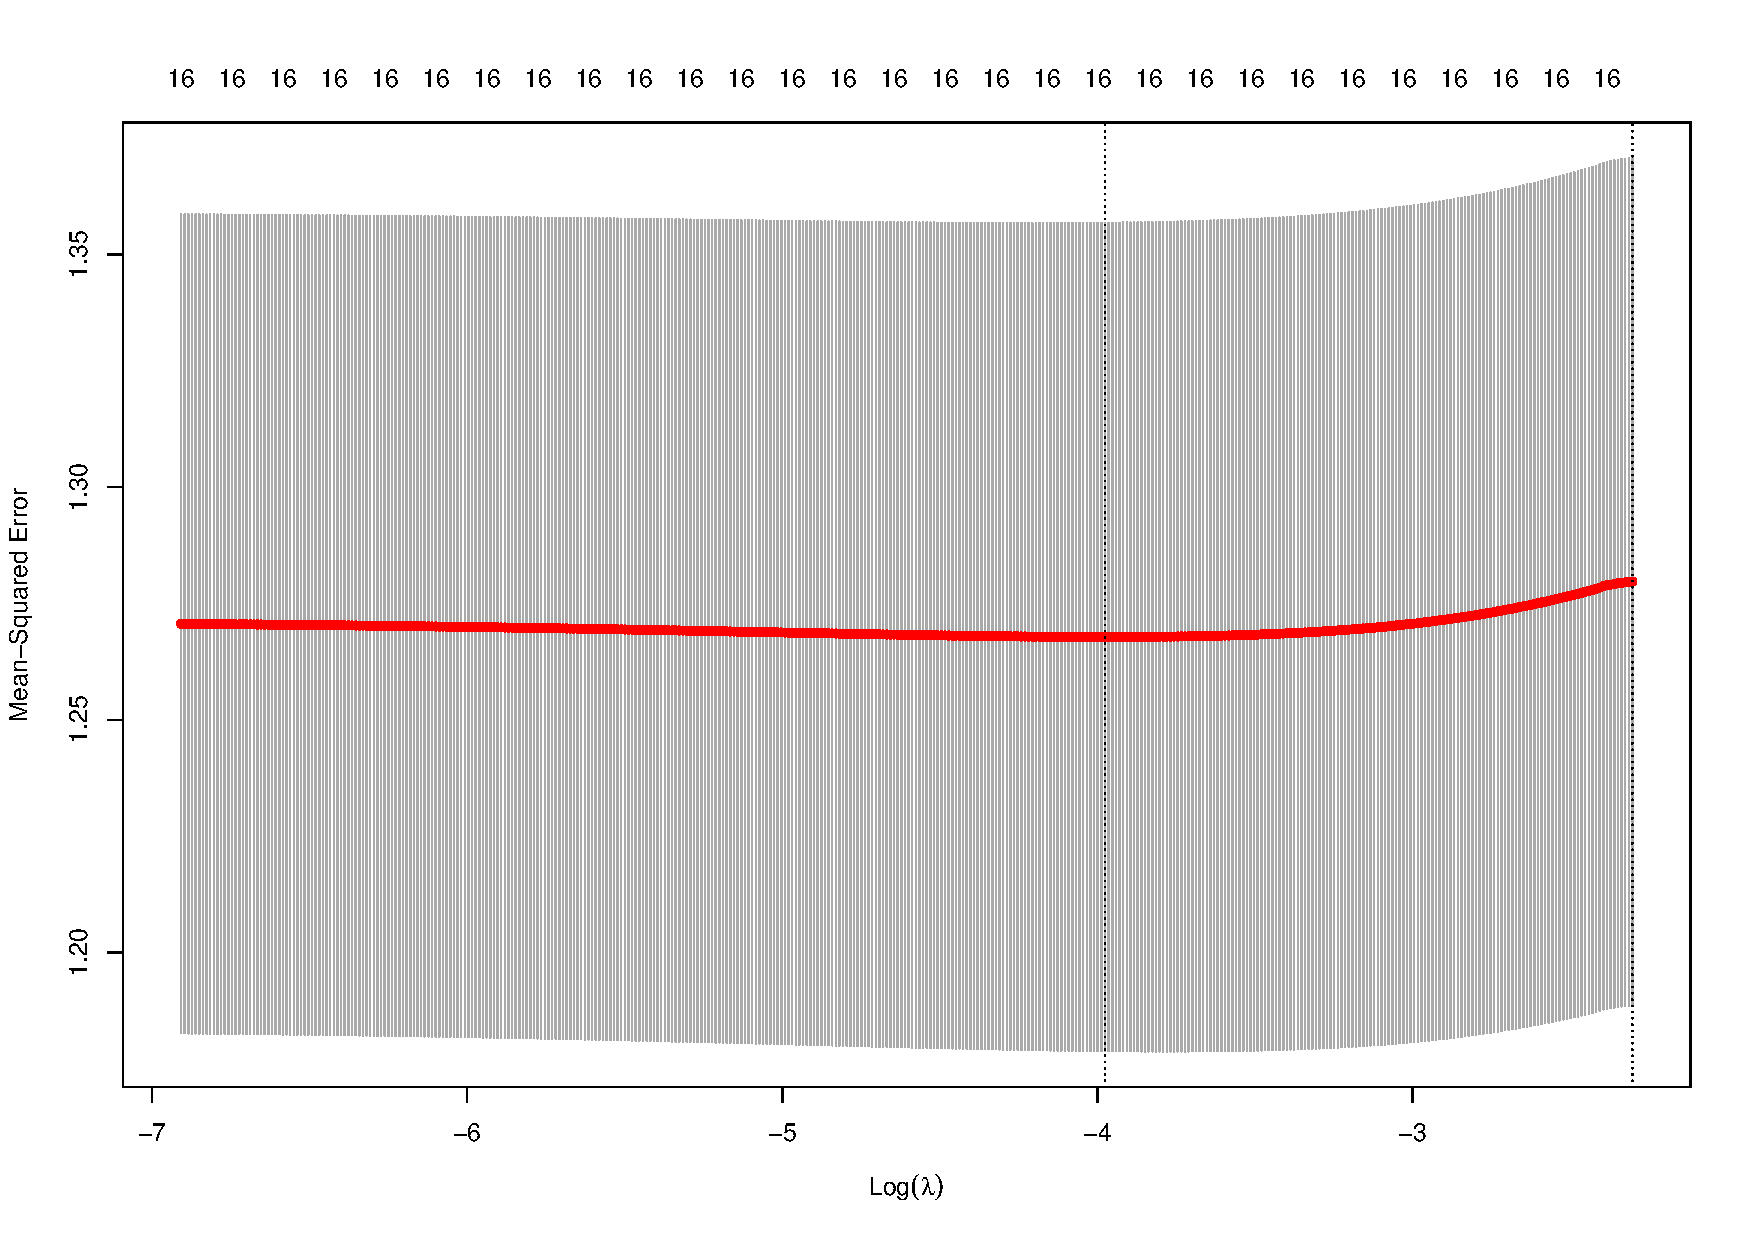
\includegraphics[width=0.7\linewidth]{ImageFiles/Regression/Ridge/RidgeCvPlot.pdf}
	\caption{Ridge cross validated MSE as function of $\lambda$.}
	\label{fig:RidgeCvPlot}
\end{figure}

We fit the final model using the optimal $\lambda$ value ($\lambda_{opt}$). The resulting coefficients are displayed in \Tab~\ref{table:FinalRidgeCoef}. For this model we computed also the test MSE and it is $MSE_{test} = 1.4234$.

In this case the ridge penalization does not reduce the number of coefficients, and it does not even improve significantly the MSE. We then can conclude that using ridge regression is not useful for our purposes.
